\chapter{The FILE menu}
%=============================================================
\begin{figure}[!htbp]
   \centering
   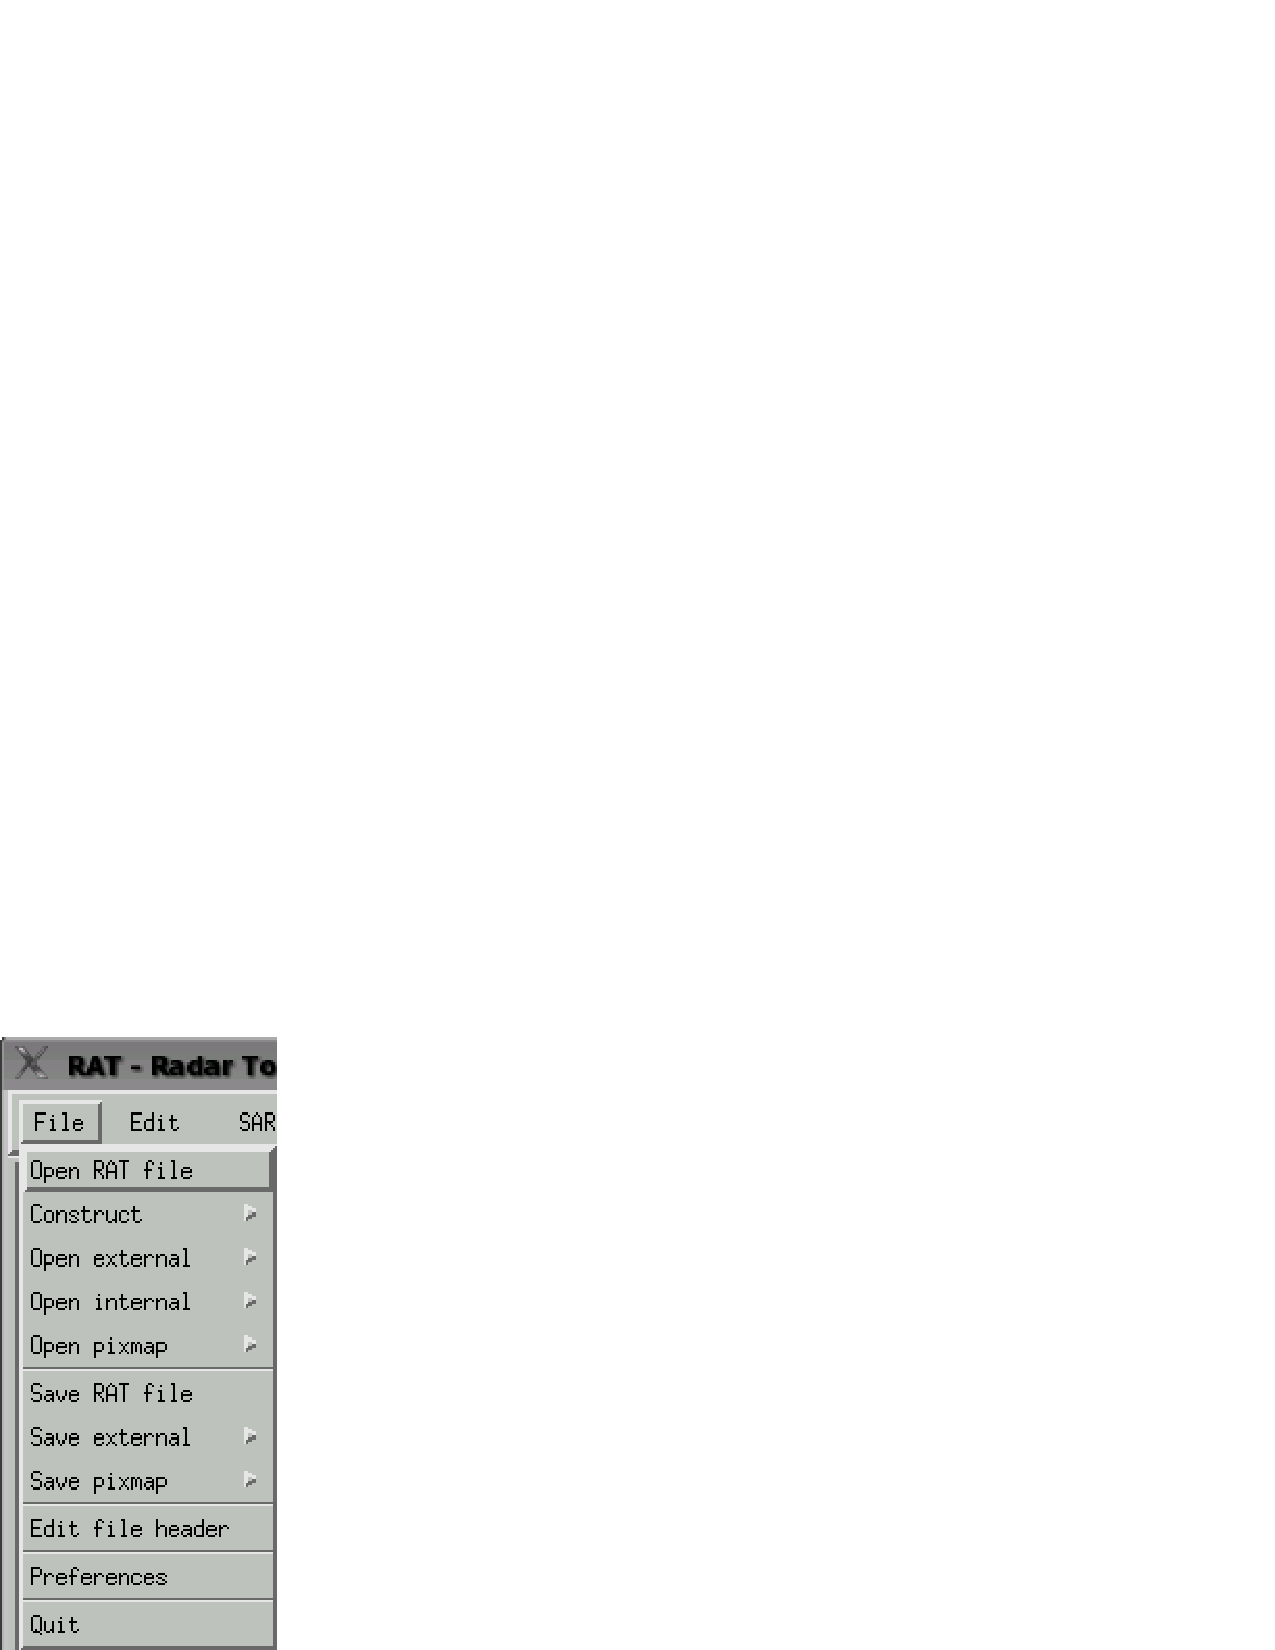
\includegraphics[scale=0.8]{images/pdf/file_menu.pdf}
\end{figure}

Use the \textbf{\textit{File}}  menu on the RAT menu bar to read files into RAT, save file, construct polarimetric or interferometric images, import or export into different data formats, set preferences, edit the file header of the RAT file format and exit RAT.

%=============================================================
\newpage 
%=============================================================
%=============================================================
\section{Open RAT file}
Use the ``Open RAT file'' to open data saved in RAT format.

\subsection{RAT file format}

RAT uses a special file format, containing information about data type, size and representation. Until some import filters are available, you'll have to convert your data to RAT format before beeing able to work with it. This is quite simple if you know how to use IDL. If not, have a look at the format description. In fact, the RAT format is just a simple header plus the data in binary representation.

\subsection{How to generate a file in RAT format with IDL}

Quite easy:
 
\begin{itemize}
	\item Enter IDL
	\item Compile RAT or restore the IDL save-file. This makes a routine for writing RAT files available (srat).
	\item Read your data into an IDL variable using your own rotines. You should know how....
	\item Write the RAT file with the command \verb*|srat,"file.rat",var| on the IDL command line. 'file.rat' denotes the RAT file to be generated, `var' the variable in which contains your data.
	\item Now you can start RAT and load the content of the file  with File$>$Open RAT file.
\end{itemize} 

\subsection{RAT format description}

A RAT-file is structured as in the following:

\begin{center}
\begin{tabular}{|c|c|p{10cm}|}
\hline 
Element & \textbf{type} & \textbf{Description} \\ 
\hline
\hline
DIM & 1*long integer & Number of dimensions of the array \\
\hline
SIZE & DIM*long integer & Array sizes for each dimension \\
\hline
VAR & 1*long integer & Type of Array (1=byte, 2=int, 3=long, 4=float, 5=double, 6=complex, 9=double complex) \\
\hline
TYPE & 1*long integer & Type of Data (100 = SAR amplitude image, 101 = SAR complex image, etc.... (see definitions.pro) \\
\hline
DUMMY & 3*long integer & Reserved \\
\hline
INFO & 80*byte & Comment string \\
\hline
ARRAY & Array type & The array itself \\
\hline 
\end{tabular}\\
\end{center}

%=============================================================
\newpage 
%=============================================================
%=============================================================
\section{Construct}
\subsection{InSAR pair}
\subsection{PolSAR pair}

%=============================================================
\newpage 
%=============================================================
%=============================================================
\section{Open external}
\subsection{E-SAR (DLR)}
\subsection{ENVISAT-ASAR}
\subsection{Radarsat-2}
This routine is made for importing RADARSAT-2 data in Geo-TIFF format into RAT.
Up to now, it has been only tested using simulated data - RADARSAT-2 is not yet
in space!

Basically, this routine has only two options: Reading quad-pol data, i.e. data
composed out of the four polarisation HH,VV,HV and VH, or single-pol data. Since
RAT does not support partial polarimetry, dual-pol data are threated as two
individual single-pol files. When reading quad-pol data, only one of the four files
has to be selected in the fileselector. RAT will automatically find the 3 others.
When not all the 4 files are found, RAT switches back to single-pol.

Many thanks to Daniel De Lisle from CSA for providing a CD with simulated sample
data.

\subsection{PolSARPro}
\subsection{Generic binary}
\subsection{ENVI standard}

%=============================================================
\newpage 
%=============================================================
%=============================================================
\section{Open internal}
\subsection{rarr / sarr}
\subsection{2*long + complex}
\subsection{E-SAR-RK (Rolf)}

%=============================================================
\newpage 
%=============================================================
%=============================================================
\section{Open pixmap}
\subsection{Open PNG}
\subsection{Open JPEG}
\subsection{Open TIFF}

%=============================================================
\newpage 
%=============================================================
%=============================================================
\section{Save RAT file}

%=============================================================
\newpage 
%=============================================================
%=============================================================
\section{Save external}
\subsection{ENVI Standard}
\subsection{Generic binary}

%=============================================================
\newpage 
%=============================================================
%=============================================================
\section{Save pixmap}
\subsection{Save PNG}
\subsection{Save JPEG}
\subsection{Save TIFF}

%=============================================================
\newpage 
%=============================================================
%=============================================================
\section{Edit file header}

%=============================================================
\newpage 
%=============================================================
%=============================================================
\section{Preferences}

%=============================================================
\newpage 
%=============================================================
%=============================================================
\section{Quit}

%  
%  %=============================================================
%  \newpage 
%  %=============================================================
%  %=============================================================
%  %=============================================================
%  \section*{Construct}
%  \addcontentsline{toc}{section}{Construct}
%  
%  \begin{center}
%  
\includegraphics[scale=1]{images/pdf/construct.pdf}
%  \end{center}
%  
%  There are two options for this menu:
%  
%  \begin{itemize}
%  \item Construct InSAR pair, to generate an interferometric data vector
%  
%  \item Construct PolSAR vector, to generate an polarimetric data vector
%  \end{itemize}
%  
%  %=============================================================
%  \newpage 
%  %=============================================================
%  %=============================================================
%  %=============================================================
%  \section*{Construct InSAR pair}
%  \addcontentsline{toc}{section}{Construct InSAR pair}
%  
%  \begin{center}
%  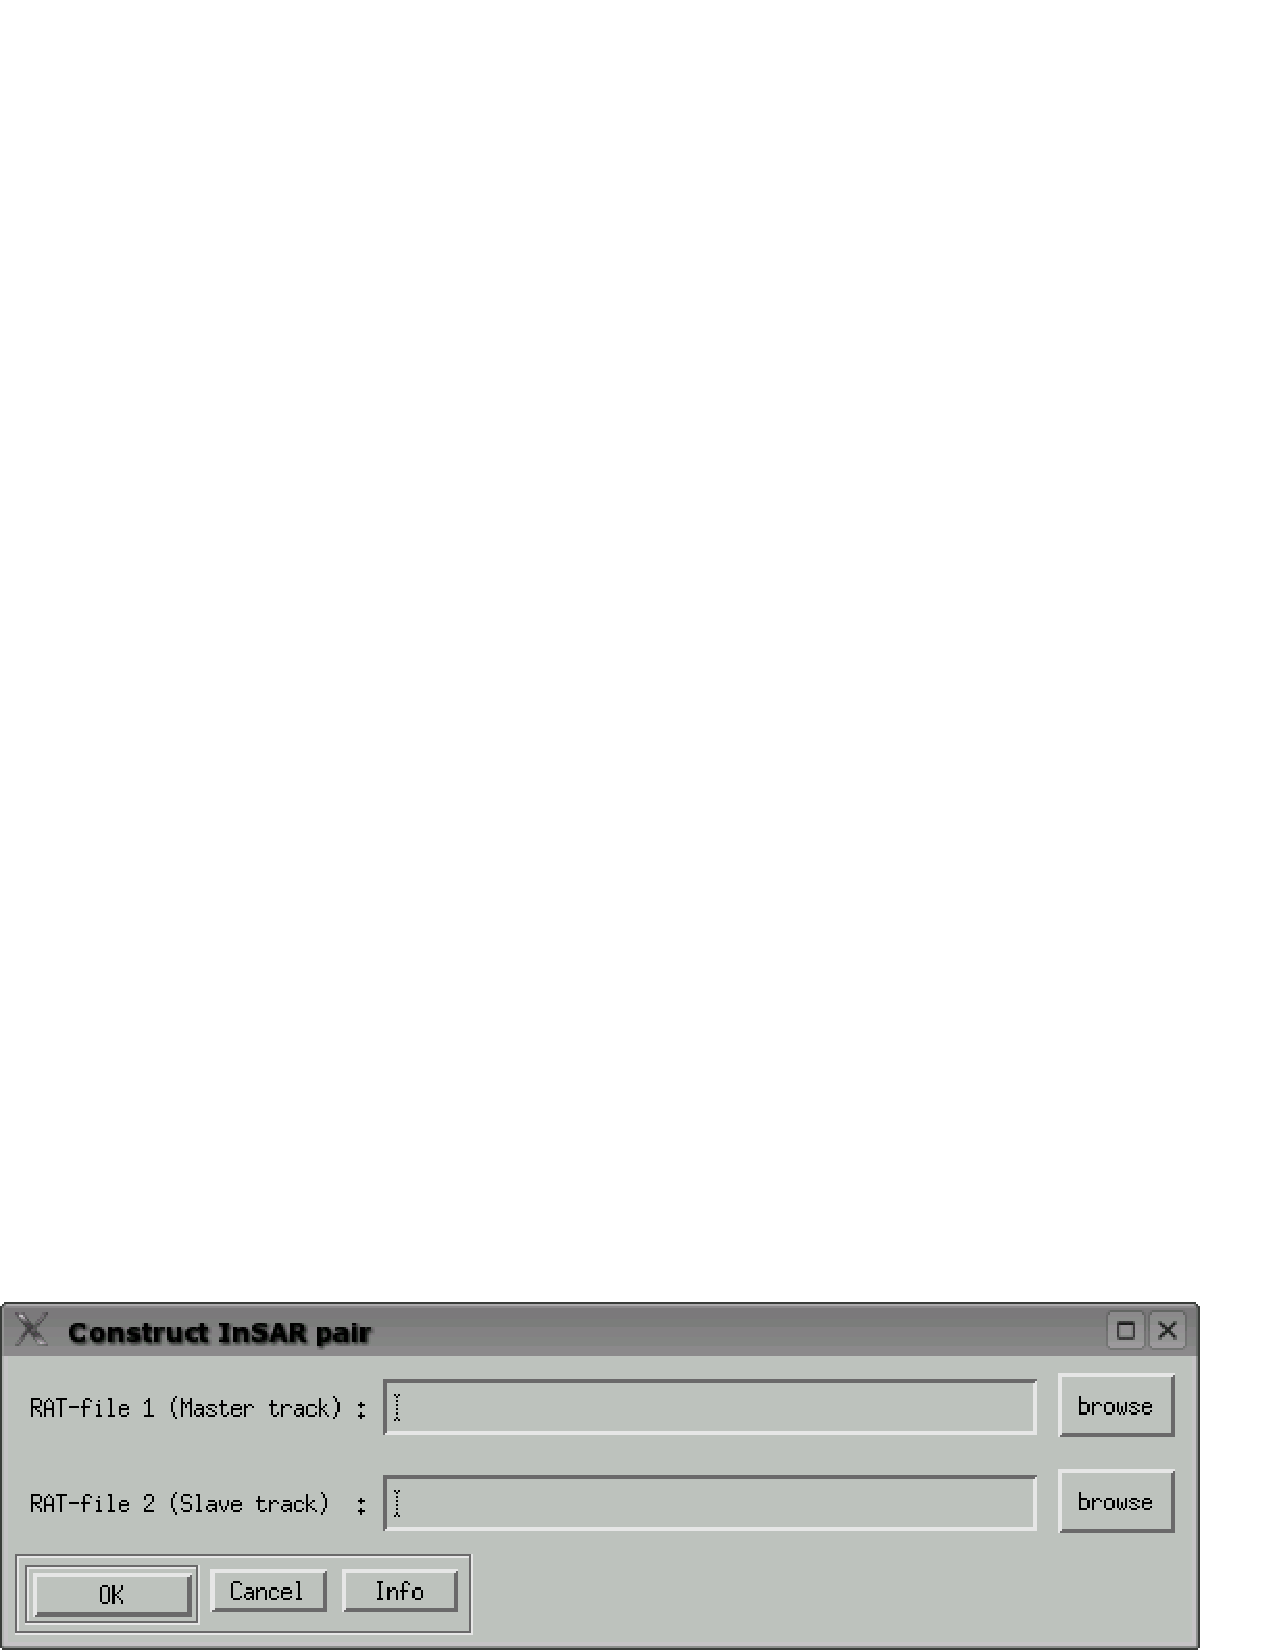
\includegraphics[scale=0.8]{images/pdf/construct_insar.pdf}
%  \end{center}
%  
%  To construct an InSAR pair data, you need two SAR images. The input files have to be in the RAT format, otherwise you will get an error message.
%  
%  The first file correponds to the reference interferometric track, also called ``master track'' and the second file corresponds to the dependant file, also called ``slave track''. 
%  
%  %=============================================================
%  \newpage 
%  %=============================================================
%  %=============================================================
%  %=============================================================
%  \section*{Construct PolSAR vector}
%  \addcontentsline{toc}{section}{Construct PolSAR vector}
%  
%  \begin{center}
%  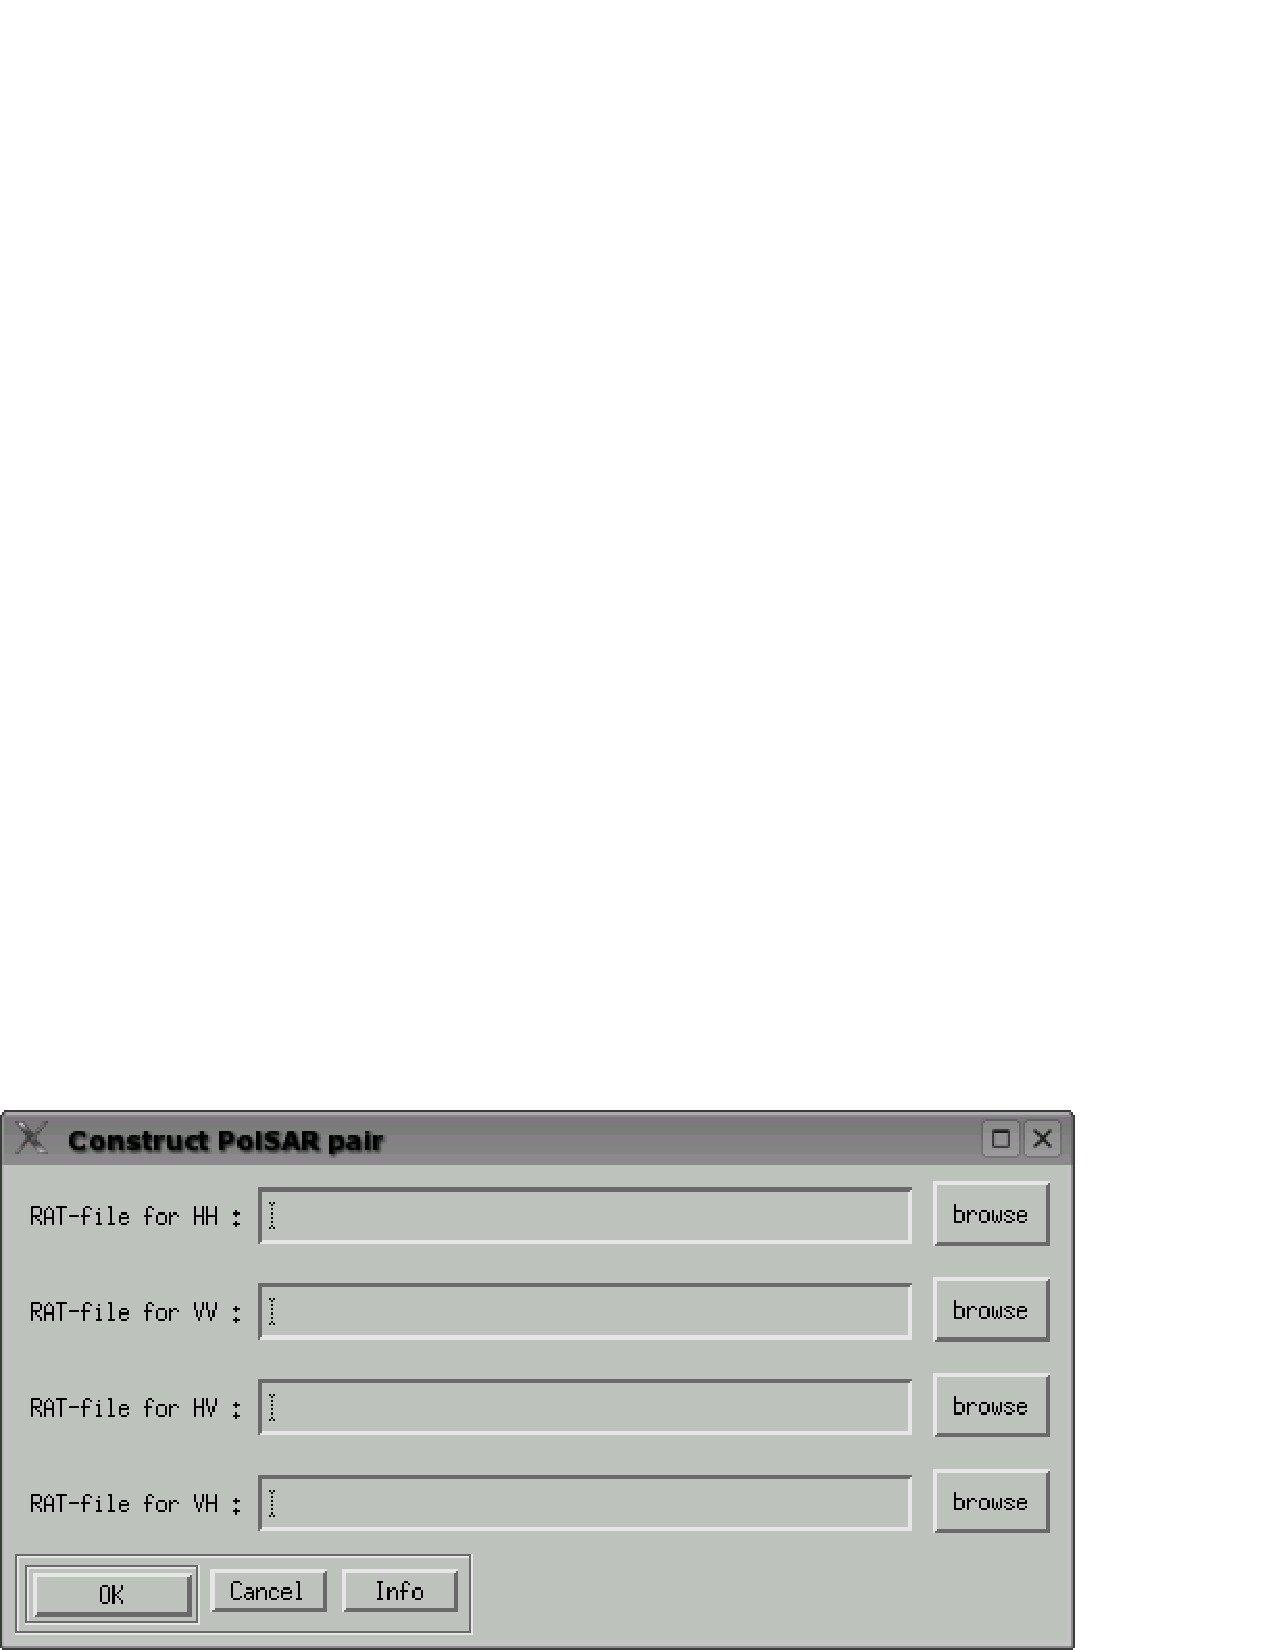
\includegraphics[scale=0.8]{images/pdf/construct_polsar.pdf}
%  \end{center}
%  
%  To construct a PolSAR vector you need, at least, 2 SAR images. The input files have to be in the RAT format, otherwise you will get an error message.
%  
%  The two first RAT--file are obligatory. By construction of RAT, the polarisation channel used should be in the horizontal/vertical basis. The first file is in polarisation HH and the second file is in polarisation VV.
%  
%  The two last files are optional. First you can add a HV channel, then, a VH channel.
%  
%  %=============================================================
%  \newpage 
%  %=============================================================
%  %=============================================================
%  %=============================================================
%  \section*{Open external}
%  \addcontentsline{toc}{section}{Open external}
%  
%  \begin{center}
%  
\includegraphics[scale=1]{images/pdf/open_external.pdf}
%  \end{center}
%  
%  There are five options for this menu:
%  
%  \begin{itemize}
%  \item E--SAR (DLR): open file data provided by the E--SAR sensor from the DLR.
%  
%  \item ENVISAT--ASAR: open file data provided by ENVISAT--ASAR.
%  
%  \item POLSARPRO: open file data provided by the software POLSARPRO
%  
%  \item Generic binary: open generic data file. You can specify lot of parameters
%  
%  \item ENVI standart: open envi standart file (only envi standart file)
%  \end{itemize}
%  
%  %=============================================================
%  \newpage 
%  %=============================================================
%  %=============================================================
%  %=============================================================
%  \section*{Open ESAR}
%  \addcontentsline{toc}{section}{Open ESAR}
%  
%  This option allows you to open a SAR data processed by the DLR. This function is based on filename analysis.
%  
%  If the format is recognise, the procedure function ask you for different more informations.
%  
%  %=============================================================
%  \newpage 
%  %=============================================================
%  %=============================================================
%  %=============================================================
%  \section*{Open ENVISAT--ASAR}
%  \addcontentsline{toc}{section}{Open ENVISAT--ASAR}
%  
%  This option allows you to open an ENVISAR--ASAR data format. These files have this \verb*|ASA*.N1| extension.
%  
%  Up to now only ASA--IMS files are supported.
%  
%  %=============================================================
%  \newpage 
%  %=============================================================
%  %=============================================================
%  %=============================================================
%  \section*{Open POLSARPRO}
%  \addcontentsline{toc}{section}{Open POLSARPRO}
%  
%  This option allows you to open file generated by the ``\textbf{POLSARPRO}'' sofware. You have to search for a config file called \verb*|config.txt|. POLSARPRO files are organised into different folders with specific name, do not change the folder name provided by POLSARPRO.
%  
%  %=============================================================
%  \newpage 
%  %=============================================================
%  %=============================================================
%  %=============================================================
%  \section*{Open Generic binary}
%  \addcontentsline{toc}{section}{Open Generic binary}
%  
%  When you choose \verb*|Open Generic Binary| the following window appears.
%  
%  \begin{center}
%  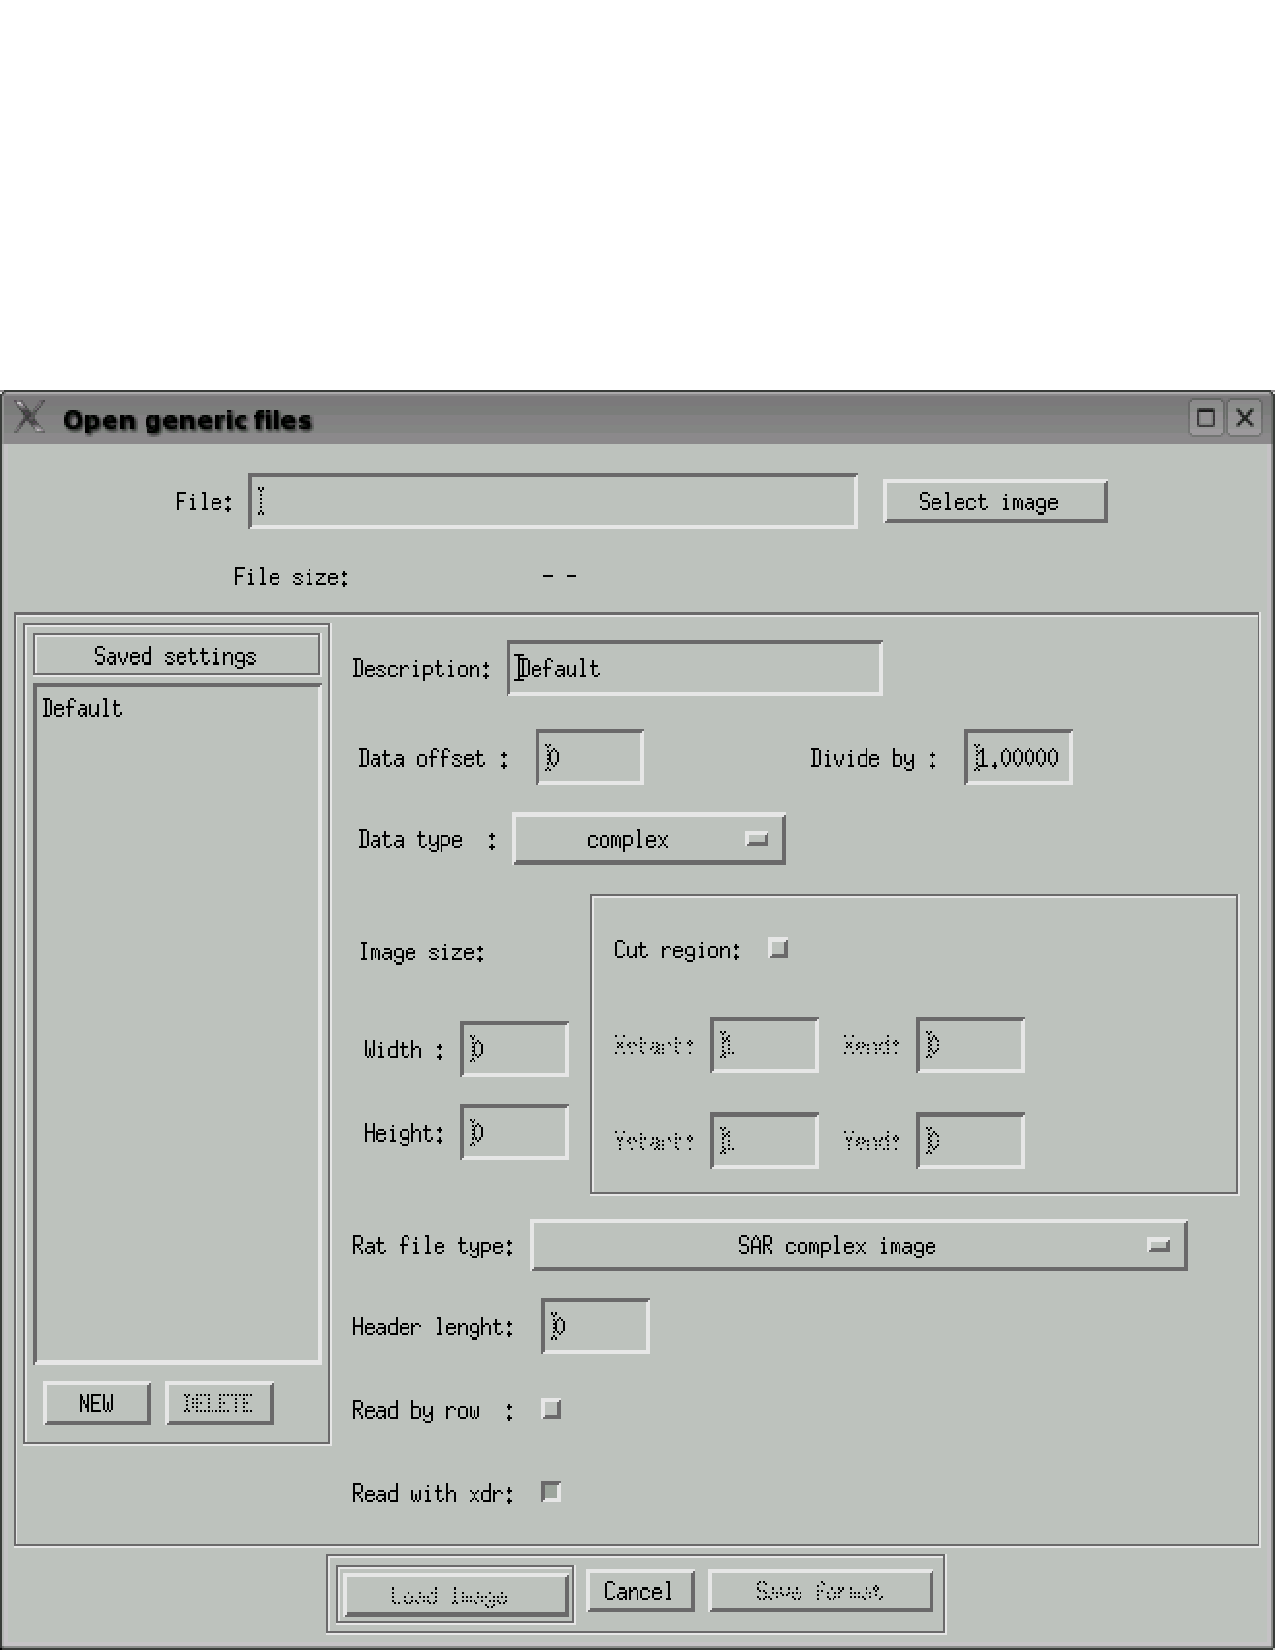
\includegraphics[scale=0.8]{images/pdf/import_gen.pdf}
%  \end{center}
%  
%  In this case, you have to specify:
%  
%  \begin{itemize}
%  
%  \item File: using the \verb*|Select image| button. At this point it will give you the size of the image.
%  
%  \item Description: you can choose a description name for you configuration if you have more than one file to open using \verb*|Open Generic Binary|. On the left side you can manage your different configuration.
%  
%  \item Data offset: you can add an global offset for all your data $new data = data + offset$.
%  
%  \item Divide by: you can divide the data by a global value.
%  
%  \item Data type: you can choose between the different kind of data existing.
%  
%  \item Image size: you have to specify the size of the image.
%  
%  \item Cut region: if you want to extract a sub image.
%  
%  \item Rat file type: define the type of file. Look at the chapter \ref{chapter:data_type} for more information.
%  
%  \item Header lenght: if your data have a header, you can specify here the lenght.
%  
%  \item Read by row: ???
%  
%  \item Read with \verb*|XDR|: allow to use the \verb*|/XDR| keyword when reading the data.
%  
%  \end{itemize}
%  
%  %=============================================================
%  \newpage 
%  %=============================================================
%  %=============================================================
%  %=============================================================
%  \section*{Open ENVI standart}
%  \addcontentsline{toc}{section}{Open ENVI standart}
%  
%  The standart ENVI file header (with \verb*|*.hdr| extension) has the following form:
%  
%  \begin{verbatim}
%  ENVI
%  description = {
%  unknown content.}
%  samples = 512
%  lines   = 512
%  bands   = 1
%  header offset = 0
%  file type = ENVI Standard
%  data type = 4
%  interleave = bip
%  sensor type = Unknown
%  byte order = 1
%  \end{verbatim}
%  
%  please, note that \verb|ENVI Standart| is specified to the \verb|file type| field.
%  
%  Up to now, only this header file is readable by RAT.
%  
